\documentclass[a4paper]{article}

\usepackage{amsmath}
\usepackage{amssymb}
\usepackage{stellar}
\usepackage{parskip}
\usepackage{fullpage}
\usepackage{wrapfig}
\usepackage{tikz}

\usetikzlibrary{arrows}
\usetikzlibrary{decorations.pathreplacing}

\title{Fisica I}
\author{Paolo Bettelini}
\date{}

% libri
% Rosati

\begin{document}

\maketitle
\tableofcontents

\section{Introduzione}

\section{Vettori spostamento}

\begin{itemize}
    \item vettore spostamento: direzione, verso, lunghezza;
    \item somma di vettori;
    \item moltiplicazione con scalare reale \(\vec{a} + (-\vec{a}) = \vec{0}\);
    \item modulo di un vettore;
\end{itemize}

\sproposition{Proprietà distributiva del prodotto rispetto alla somma vettoriale}{
    \[\alpha(\vec{a} + \vec{b}) = \alpha\vec{a} + \alpha\vec{b}\]
}

\section{Sistemi di coordinate}

Il punto di origine è il posto in cui viene posizionato l'osservatore.
I sistemi di coordinate trattati sono esclusivamente cartesiani e con basi ortogonali.
L'oservatore ha i versori delle direzioni.

Si possono quindi individuare le componenti di un vettore lungo le sue direzioni, ossia
le proiezioni ortogonali del vettori lungo gli assi cartesiani.
Di conseguenza, le coordinate di un vettore hanno senso solamente rispetto ad una base.

\sdefinition{Prodotto scalare}{
    Il prodotto scalare fra due vettori risulta in un numero reale (in uno spazio euclideo \(\mathbb{R}^n\))
    \[
        \vec{a} \cdot \vec{b} \in \mathbb{R}
    \]
    Dato l'angolo \(\theta\) fra \(\vec{a}\) e \(\vec{b}\),
    \[
        \vec{a}\cdot \vec{b} = |\vec{a}| \cdot|\vec{b}| \cdot \cos\theta
    \]
}

Chiaramente il prodotto scalare è commutativo.

\sproposition{Proprietà distributiva del prodotto scalare rispetto alla somma}{
    \[
        \vec{c} \cdot (\vec{a} + \vec{b}) = c\vec{a} + c\vec{b}
    \]
}

\sproposition{Prodotto vettoriale con componenti}{
    TODO....
}

Da qui possiamo notare che il prodotto scalare ha lo stesso ridultato per ogni basta ortonormata.

% fai il prodotto fra c e a+b, e poi espandi la distributiva e semplifica i termini ortogonali.

\sdefinition{Prodotto vettoriale}{
    Il prodotto scalare fra due vettori risulta in un vettore (in uno spazio euclideo \(\mathbb{R}^n\))
    \[
        \vec{a} \wedge \vec{b} \in \mathbb{R}
    \]
    Dato l'angolo \(\theta\) fra \(\vec{a}\) e \(\vec{b}\),
    il risultato è un vettore con modulo
    \[
        |\vec{a} \wedge \vec{b}| = |a||b|\sin\theta
    \]
    e direzione normale al piano formato da \(\vec{a}\) e \(\vec{b}\).
    Convenzionalmente, il verso del vettore normale è scelto secondo 
    la regola della mano destra.
}

\sproposition{Proprietà del prodotto vettoriale}{
    \begin{enumerate}
        \item \(\vec{a} \wedge \vec{b} = - \vec{b} \wedge \vec{a}\);
        \item \((\gamma \vec{a}) \wedge \vec{b} = \gamma (\vec{a} \wedge \vec{b})\);
        \item \((\vec{a} + \vec{b}) \wedge \vec{c} = \vec{a} \wedge \vec{c} + \vec{b} \wedge \vec{c}\)
    \end{enumerate}
}

Consideriamo \(\vec{a}\) e \(\vec{b}\), allora
\begin{align*}
    \vec{a} &= a_x\hat{x} + a_y\hat{y} + a_y\hat{z} \\
    \vec{b} &= b_x\hat{x} + b_y\hat{y} + b_y\hat{z}
\end{align*}
Sapendo che
\begin{align*}
    \hat{x} \wedge \hat{y} &= \hat{z} \\ 
    \hat{x} \wedge \hat{z} &= -\hat{y} \\
    \hat{y} \wedge \hat{z} &= \hat{x} \\
\end{align*}
Possiamo eseguire il prodotto esplicitamente
\begin{align*}
    \vec{a} \wedge \vec{b} &= a_xb_y\hat{z} + a_xb_z(-\hat{y}) + a_yb_x(-\hat{z})
    + a_yb_z\hat{x} + a_zb_x\hat{y} + a_zb_y(-\hat{x}) \\
    &= \left[a_yb_z - a_zb_z\right] \hat{x} + \left[a_zb_x - a_xb_z\right]\hat{y}
    + \left[a_xb_y - a_yb_x\right] \hat{z}
\end{align*}

\pagebreak

\section{Cinematica}

La cinematica è la parte della meccanica che descrive il moto di un punto materiale.
Per descrivere il moto di un oggetto è necessario procurarsi un sistema di riferimento.
Sceglieremo quindi un'origine e una base ortonormata.

\sdefinition{Posizione}{
    La \textit{posizione} di un punto è rappresentata unicamente da un vettore \(\vec{r}(t)\),
    che mostra lo spostamento fra l'origine e la sua posizione \(P(t)\) in un determinato istante di tempo.
}

Se vogliamo considerare la posizione solo nella direzione \(x\)
possiamo calcoalre
\[
    \hat{x}(t) = \vec{x}\vec{r}(t)
\]
In generale
\[
    \vec{r}(t) = \hat{x}\vec{r}(t) + \hat{x}\vec{y}(t) + \hat{z}\vec{r}(t)
\]

La relazione fra due osservatori diversi è data da \(\vec{R} + \vec{r'}(t) = \vec{r}(t)\).

La velocità è quindi relativa a due posizioni \(P(t)\) e \(P(t + \Delta t)\).
Lo spostamento è \(\vec{r}(t + \Delta t) = \vec{r}(t) + \vec{s}(t)\).

\sdefinition{Velocità}{
    La \textit{velocità} di un punto rappresenta lo spostamento che il punto materiale
    percorre in un unità di tempo \(\vec{v}(t)\).
    Allora la velocità è definita come
    \[
        \vec{v}(t) = \lim_{\Delta t \to 0} \frac{\vec{s}}{\Delta t}
        = \lim_{\Delta t \to 0} \frac{\vec{r}(t+\Delta t) - \vec{r}(t)}{\Delta t}
        = \frac{d\vec{r}(t)}{dt}
    \]
}

Il vettore della velocità si orienta verso la tangente della curva (cioè nella direzione in cui si sta spostando).
Chiaramente la derivata può essere separata nelle componenti
\[
    \vec{v}(t)=v_x\hat{x} + v_y\hat{y} + v_z\hat{z}
\]
dove possiamo anche dire che
\[
    v_x(t) = \frac{dx(t)}{dt}
\]

\sdefinition{Accelerazione}{
    L'\textit{accelerazione} di un punto rappresenta il cambiamento istantaneo della velocità
    \[
        \vec{a}(t) = \lim_{\Delta t \to 0} \frac{\vec{v}(t + \Delta t) - \vec{v}(t)}{\Delta t}
    \]
}

\section{Leggi orarie}

\sproposition{Caduta da una altezza}{
    Il tempo di caduta di un oggetto da un altezza \(h\), soggetto a gravità costante \(g\)
    è cado da
    \[
        t_\text{caduta} = \sqrt{\frac{2h}{g}}
    \]
    con velocità
    \[
        -\sqrt{2gh}
    \]
}

\pagebreak

\section{Moto arbitrario}

Consideriamo un moto arbitrario \(\vec{r}(t)\). Questo vettore punta sempre alla posizione dell'oggetto.
La sua velocità \(\vec{v}(t) = \frac{d\vec{r}(t)}{dt}\) è un vettore sempre nella direzione della traiettoria.
Definiamo allora il versore tangente
\[
    \hat{T}(t) v(t) = \vec{v}(t)
\]
Abbiamo allora che
\[
    \vec{a}(t) = \frac{d}{dt} \left(v(t)\hat{T}(t)\right) = \frac{dv(t)}{dt}\hat{T}(t) + v(t)\frac{d\hat{T}(t)}{dt} = a_t(t)\hat{T}(t) + v(t)\frac{d\hat{T}(t)}{dt}
\]
La prima componente, \(\frac{dv(t)}{dt}\hat{T}\), è chiamamta \textit{accelerazione tangenziale}
mentre il secondo \textit{accelerazione centripeta} (entrambi sono perpendicolari fra di loro).

Per studiare il significato di tale termine, cominciamo partendo dall'identità \(\hat{T}(t) \cdot \hat{T}(t) = 1\).
Allora,
\begin{align*}
    \frac{d}{dt} \left( \hat{T}(t) \cdot \hat{T}(t) \right) &= 0 \\
    \frac{d\hat{T}(t)}{dt} \cdot \hat{T}(t) + \hat{T}(t)\frac{d\hat{T}(t)}{dt} &= 0 \\
    \hat{T}(t)\frac{d\hat{T}(t)}{dt} &= 0 
\end{align*}
Dall'analisi differenziale troviamo che
\[
    \left|\frac{\hat{T}(t)}{dt}\right| = \lim_{\Delta t \to 0} \frac{dl}{\Delta t}
\]
e l'arco di circonferenza
\[
    s = Rd\theta
\]
dove \(R\) è la lunghezza della retta fino al punto di rotazione (raggio di curvatura, ossia il raggio del cerchio osculatore).
Mettendo assieme queste due informazioni troviamo che
\[
    \left|\frac{d\hat{T}(t)}{dt}\right| = \lim_{\Delta t \to 0} \left[\frac{S}{\Delta t} \frac{1}{R}\right] = \frac{v}{R}
\]
Adesso possiamo scrivere
\[
    \vec{a}(t) = \frac{dv}{dt}\hat{T} + v\frac{d\hat{T}}{dt} = \frac{dv}{dt}\hat{T} + \frac{v^2}{R} \hat{N}
\]
e quindi \(\frac{dv}{dt}\) è la componente tangenziale e \(\frac{v^2}{R}\) quella centripeta.
Notiamo che l'accelerazione centripeta è più piccola più il cerchio è grande, quindi nulla
quando andiamo dritti.

Nel caso specifico del moto circolare,
\[
    \vec{a} = -\omega^2\vec{r} = \frac{v^2}{R} \hat{N}
\]
con \(\omega = \frac{v}{R}\).

% derivata di prodoto scalare usa la usuale regola di derivata.

\pagebreak

\section{Relatività}

\sexercise{Moto di precessione}{
    Consider \(\vec{a}(t)\) and \(\vec{w}\) fixed with the condition that
    \[
        \frac{d\vec{a}}{dt} = \vec{w} \wedge \vec{a}
    \]
    We first note that \(|\vec{a}(t)|\) is constant.
    We have that
    \begin{align*}
        \frac{d}{dt} {|\vec{a}(t)|}^2 &= \frac{d}{dt} \vec{a}\cdot\vec{a}
        = \vec{a}\frac{d\vec{a}}{dt} + \frac{d\vec{a}}{dt} \vec{a} 
        = 2\vec{a}\frac{d\vec{a}}{dt}
        = 2 \vec{a} \cdot (\vec{w} \wedge \vec{a})
        = 0
    \end{align*}
    We define out cartesian system with the condition that \(\hat{z}\) has the direction
    direction and length as \(\vec{w}\), thus \(\vec{w} = w\hat{z}\).
    As a second fact we have that \(a_z\) is independent of time.
    Indeed,
    \[
        \frac{da_z}{dt} = \frac{d\vec{a}\hat{z}}{dt} =  \hat{z}\frac{d\vec{a}}{dt}
        = \hat{z} \cdot (\vec{\omega} \wedge \vec{a})
        = 0
    \]
    so it is constant. Geometrically, \(\vec{a}\) creates a cone.
    Now, \(\vec{a}_\perp^2 = a^2 - a_z^2\) which is independent of \(t\),
    and \(a_x = a_T \cos\phi\) where \(\phi\) is the angle between \(\hat{x}\)
    and the projection \(a_\perp\) (on the \(xy\) plane).
    \[
        \begin{cases}
            a_x(t) = a_\perp \cos\phi(t) \\
            a_y(t) = a_\perp \sin\phi(t) \\
            a_t
        \end{cases}
    \]
    We now have
    \begin{align*}
        \frac{da_x}{dt} &= {(\vec{w} \wedge \vec{a})}_x
        = -\omega a_y \\
        \frac{da_x}{dt} &= {(\vec{w} \wedge \vec{a})}_y
        = \omega a_x \\
        \frac{da_z}{dt} &= {(\vec{w} \wedge \vec{a})}_z
        = 0
    \end{align*}
    We can substitute the parametrization
    \begin{align*}
        \frac{da_x}{dt} &= -\omega a_y \implies a_\perp (-\sin(\phi(t))) \cdot \frac{d\phi}{dt} = -\omega a_\perp \sin\phi(t) \\
        \frac{da_y}{dt} &= -\omega a_x \implies a_\perp \cos(\phi(t)) \cdot \frac{d\phi}{dt} = \omega a_\perp \cos\phi(t) \\
        \frac{da_z}{dt} &= 0
    \end{align*}
    We note that simplifying these equations yields the same equation 
    \begin{align*}
        \frac{d\phi}{dt} = \omega \\
        \frac{d\phi}{dt} = \omega
    \end{align*}
    for \(a_\perp \neq 0\),
    which is obvious given the relation that we had established.
    Thus, the final solution is \(\phi(t) = \phi_0 + \omega t\).
    In conclusion,
    \[
        \begin{cases}
            a_x = a_\perp \cos(\omega t + \phi_0) \\
            a_y = a_\perp \sin(\omega t + \phi_0) \\
            a_z = a_z
        \end{cases}
    \]
}

Vogliamo mettere in relazione la descrizione del moto di un punto materiale
con le osservazioni fatte da due osservatori \(O\) e \(O'\).
Definiamo \(\vec{r}(t)\) come l'osservazione di \(O\) e \(\vec{r}'(t)\) come quella di \(O'\).
Definiamo anche \(\vec{r}(t) = \vec{R}(t) + \vec{r}'(t)\).

\begin{center}
    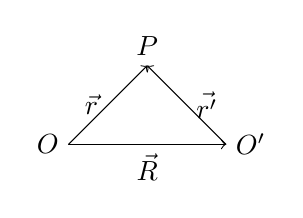
\begin{tikzpicture}[line cap=round,line join=round,scale=1]
        \coordinate (P) at (0, 1);
        \coordinate (O) at (-1, 0);
        \coordinate (Op) at (1, 0);

        \node[anchor=east] at (O) {\(O\)};
        \node[anchor=west] at (Op) {\(O'\)};
        \node[anchor=south] at (P) {\(P\)};

        \draw[->] (O) -- node[anchor=east] {\(\vec r\)} (P);
        \draw[->] (Op) -- node[anchor=west] {\(\vec {r'}\)} (P);
        \draw[->] (O) -- node[anchor=north] {\(\vec R\)} (Op);
    \end{tikzpicture}
\end{center}

Definiamo gli assi \(\hat{x}\), \(\hat{y}\) e \(\hat{z}\) per l'osservatore \(O\)
e \(\hat{u_1}\), \(\hat{u_2}\) e \(\hat{u_3}\) per \(O'\).
Chiaramente, questi versori sono dipendenti dal tempo per l'osservatore che non le usa (a meno
che i due osservatori non coincidano).
Dato questo sistema, abbiamo allora
\[
    \vec{r}'(t) = \sum_{i=1}^3 x_i'(t)\hat{u_i}(t)
\]
Abbiamo allora che
\begin{align*}
    \frac{d\vec{r}'(t)}{dt} &= \sum_{i=1}^3 \frac{dx_i'(t)}{dt} \hat{u_i}(t)
    + \frac{d\hat{u_i}(t)}{dt} x_i'(t) \\
    &= \sum_{i=1}^3 \frac{dx_i'(t)}{dt} \hat{u_i}(t)
    + \sum_{i=1}^3 \frac{d\hat{u_i}(t)}{dt} x_i'(t)
\end{align*}
The first term
\[
    \sum_{i=1}^3 \frac{dx_i'(t)}{dt} = \vec{r}'(t)
\]
is what \(O'\) perceives as the velocity, \(\vec{v}'(t)\).
Il termine dice di quanto cambiano le coordinate nel sistema di riferimento di \(O'\),
ossia la sua velocità.
Il secondo termine
\[
    \sum_{i=1}^3 \frac{d\hat{u_i}(t)}{dt} x_i'(t)
\]
compensa il primo.
Abbimo quindi che
\[
    \vec{v} = \vec{V} + \vec{v}'(t) + \sum_{i=1}^3 \frac{d\hat{u_i}(t)}{dt} x_i'(t)
\]

\stheorem{}{
    Esiste un vettore \(\vec{\omega}(t)\) tale che
    \[
        \frac{d\vec{u_i}}{dt} = \vec{w}(t) \wedge \vec{u_i}
    \]
}

Ciò vorrebbe dire che la terna di assi sta precedendo attorno alla direzione di \(\vec{\omega}\).
Tutte e 3 i versori stanno ruoando attorno allo stesso asse (infatti, non vi è l'indice \(i\) nel termine
\(\vec{\omega}\)). Tuttavia, il vettore \(\vec{\omega}\) stesso non è costante.
Per dimostrare ciò, dobbiamo dare la forma di \(\vec{\omega}\):
\[
    \vec{\omega}(t) = \frac{1}{2} \sum_{j=1}^3 \hat{u_j} \wedge \frac{d \hat{u_j}}{dt}
\]

Sostituendo otteniamo
\begin{align*}
    \vec{v} &= \vec{V} + \vec{v}'(t) + \sum_{i=1}^3 x_i'(\vec{\omega} \wedge \hat{u_i}) \\
    &= \vec{V} + \vec{v}'(t) + \vec{\omega} \wedge \sum_{i=1}^3 x_i'\hat{u_i} \\
    &= \vec{V} + \vec{v}'(t) + \vec{\omega} \wedge \vec{r}'(t)
\end{align*}

Verifichiamo che la forma di \(\vec{\omega}\) soddisfi la condizione data, quindi
\begin{align*}
    (\vec{\omega} \wedge \hat{u_i})_x &= \omega_y u_i^z - \omega_z u_i^y \\
    &= \frac{1}{2} \sum_{j=1}^3 \left\{ u_i^z \left[u_j^z \frac{du_j^x}{dt} - u_j^x \frac{du_j^z}{dt}\right]
     - u_i^y \left[u_j^x \frac{du_j^y}{dt} - u_j^y \frac{du_j^x}{dt}\right] \right\} \\
     &= \frac{1}{2} \sum_{j=1}^3 \left\{
        \frac{du_j^x}{dt} \left[
            u_i^z u_j^z + u_i^yu_j^y
        \right]
        - \frac{du_j^y}{dt} u_i^yu_j^x - \frac{du_j^z}{dt} u_i^zu_j^x
     \right\} \\
     &= \frac{1}{2} \sum_{j=1}^3 \left\{
        \frac{du_j^x}{dt} \left[
            \hat{u_i} \cdot \hat{u_j} - u_i^x u_j^x
        \right]
        - \frac{du_j^y}{dt} u_i^yu_j^x - \frac{du_j^z}{dt} u_i^zu_j^x
     \right\} \\
     &= \frac{1}{2} \sum_{j=1}^3 \left\{
        \frac{du_j^x}{dt} \left[
            \delta_{i,j} - u_i^x u_j^x
        \right]
        - \frac{du_j^y}{dt} u_i^yu_j^x - \frac{du_j^z}{dt} u_i^zu_j^x
     \right\} \\
     &= \frac{1}{2} \sum_{j=1}^3 \left\{
        \frac{du_j^x}{dt} \delta_{i,j} - u_j^x \left[
            u_i^x \frac{du_j^x}{dt} + \frac{du_j^y}{dt} u_i^y + \frac{du_j^z}{dt} u_i^z
        \right]
     \right\} \\
     &= \frac{1}{2} \frac{du_i^x}{dt} - \frac{1}{2} \sum_{j=1}^3
        u_j^x \left[
            u_i^x \frac{du_j^x}{dt} + \frac{du_j^y}{dt} u_i^y + \frac{du_j^z}{dt} u_i^z
        \right] \\
    &= \frac{1}{2} \frac{du_i^x}{dt} - \frac{1}{2} \sum_{j=1}^3
        u_j^x \left[
            \hat{u_i} \cdot \frac{d\hat{u_j}}{dt}
        \right]
\end{align*}

Siccome
\[
    0 = \frac{\hat{u_i}}{dt} \cdot \hat{u_j} + \hat{u_i} \frac{\hat{u_j}}{dt}
\]
Allora
\[
    \hat{u_i} \frac{\hat{u_j}}{dt} = - \frac{\hat{u_i}}{dt} \cdot \hat{u_j}
\]
e quindi
\begin{align*}
    (\vec{\omega} \wedge \hat{u_i})_x &= \omega_y u_i^z - \omega_z u_i^y \\
    &= \frac{1}{2} \frac{du_i^x}{dt} + \frac{1}{2} \sum_{j=1}^3
    u_j^x \left[
        \hat{u_j} \cdot \frac{d\hat{u_i}}{dt}
    \right] \\
    &= \frac{1}{2} \frac{du_i^x}{dt} + \frac{1}{2} \frac{du_i^x}{dt} \\
    &= \frac{du_i^x}{dt}
\end{align*}

Abbiamo quindi che
\[
    (\vec{\omega} \wedge \hat{u_i})_x = \frac{du_i^x}{dt}
    \qquad
    (\vec{\omega} \wedge \hat{u_i})_y = \frac{du_i^y}{dt}
    \qquad
    (\vec{\omega} \wedge \hat{u_i})_z = \frac{du_i^z}{dt}
\]

Tornando alla velocità,
\begin{align*}
    \vec{v} &= \vec{V} + \vec{v}' + \sum_{i=1}^3 x_i' (\vec{\omega} \wedge \hat{u_i}) \\
    &= \vec{V} + \vec{v}' + \vec{\omega} \wedge \sum_{i=1}^3 x_i' \hat{u_i} \\
    &= \vec{V} + \vec{v}' + \vec{\omega} \wedge \vec{r}'
\end{align*}

Troviamo ora la medesima relazione per l'accelerazione.
Siccome
\begin{align*}
    \frac{d\vec{v}'}{dt} &= \sum_{i=1}^3 \left[
        \frac{d^2 x_i'}{dt^2} \hat{u_i} + \frac{dx_i'}{dt} \frac{d\hat{u_i}}{dt}
    \right] \\
    &= \vec{a}' + \sum_{i=1}^3 \frac{dx_i'}{dt} \frac{d\hat{u_i}}{dt} \\
    &= \vec{a}' + \sum_{i=1}^3 \frac{dx_i'}{dt} (\vec{\omega} \wedge \hat{u_i}) \\
    &= \vec{a}' + \vec{\omega} \wedge \sum_{i=1}^3 \frac{dx_i'}{dt} \hat{u_i} \\
    &= \vec{a}' + \vec{\omega} \wedge \vec{v}'
\end{align*}
Possiamo trovare la velocità
\begin{align*}
    \vec{a} &= \vec{A} + \frac{d\vec{v}'}{dt} + \frac{d\vec{\omega}}{dt} \wedge \vec{r}'
    + \vec{\omega} \wedge \frac{d\vec{r}'}{dt} \\
    &= \vec{A} + \vec{a}' + 2 \vec{\omega} \wedge \vec{v}' + \frac{d\vec{\omega}}{dt} \wedge \vec{r}'
    + \vec{\omega} \wedge (\vec{\omega} \wedge \vec{r}')
\end{align*}

L'ultimo termine \(\vec{\omega} \wedge (\vec{\omega} \wedge \vec{r}')\) è l'accelerazione centrifuga.
Il termine \(2 \vec{\omega} \wedge \vec{v}'\) è l'accelerazione di Coriolis.

\pagebreak

\section{Dinamica}

\textbf{Principio di relatività:}
Non esiste nessun esperimento in grado di decidere se noi siamo in quiete rispetto allo spazio assoluto
o ci stiamo muovendo in un moto rettilineo uniforme. Alternativamente, tutte le leggi della fisica sono equivalenti
indipendentemente dalla direzione dell'esperimento e dal sistema di riferimento (inerziali).

Il principio della relavitià risale a Galileo nel dialogo, 1632.

\textbf{Leggi di Newton:}
\begin{enumerate}
    \item un corpo mantiene il prorpio stato di quiete
    o di moto rettilineo uniforme
    se non agiscono forze esterne;
    \item \(\vec{F} = m\vec{a}\);
    \item se un corpo \(1\) esercita una forza \(\vec{F_{1,2}}\) su un corpo \(2\),
    allora il corpo \(2\) esercita una forza \(\vec{F_{2,1}} = -\vec{F_{1,2}}\)
    sul corpo \(1\).
\end{enumerate}

La prima è in realtà un caso particolare della seconda.

L'espressione \(\vec{F} = m\vec{a}\) è una relazione fra causa ed effetto. La forza è la causa,
che determina direttamente le accelerazioni.

Tuttavia, è necessario prima definire il concetto di massa.
Ciò può essere fatto con una serie di esperimenti e osservazioni.
Consideriamo due palline attaccate ai capi di una molla:
\begin{enumerate}
    \item \(\vec{a_1} \neq 0 \implies \vec{a_2} \neq 0\);
    \item \(\vec{a_1}\) e \(\vec{a_2}\) hanno verso opposto;
    \item il rapporto \[
        \frac{|\vec{a_1}|}{|\vec{a_2}|}
    \]
    è indipendente dalla interazione, bensì solamente dalle caratteristiche
    delle particelle;
    \item se i due corpi sono dello stesso materiale, ma di volumi diversi,
    allora
    \[
        \frac{|\vec{a_1}|}{|\vec{a_2}|} = \frac{V_2}{V_1}
    \]
\end{enumerate}
Allora, per ogni coppia di corpi, definiamo
\[
    \frac{m_2}{m_1} = \frac{|\vec{a_1}|}{|\vec{a_2}|}
\]
Dobbiamo quindi scegliere una massa di base sulla quale basare le altre misure.
Sperimentalmente, troviamo anche che \(\vec{F_1} + \vec{F_2} = m(\vec{a_1} + \vec{a_2})\).

Conservazione della quantità di moto
\[
    \vec{Q} = m\vec{v}
\]
e
\[
    \vec{Q} = \vec{Q_1} + \vec{Q_2} = m_1\vec{v_1} +  m_2\vec{v_2}
\]
La derivata della quantità di moto è data da
\[
    \frac{d\vec{Q}}{dt} = m_1 \frac{d\vec{v_1}}{dt} + m_2 \frac{d\vec{v_2}}{dt}
    = m_1 \vec{Q_1} + m_2 \vec{Q_2}
\]
Il vettore della quantità di moto nel tempo, di due moti che interagiscono fra di loro,
è sempre il medesimo, e quindi si conserva.

\pagebreak

\section{Forze elastiche (Legge di Hooke)}

\stheorem{Legge di Hooke}{
    La forza elastica è data da
    \[
        \vec{F_e} = -k \vec{x}
    \]
    dove \(\vec{x}\) è il vettore di elongazione e
    \(k\) è la costante elastica.
    Il segno negativo indica che la forza è una forza di richiamo.
}

In realtà questa è un'approssimazione lineare,
e presume quindi che lo spostamento sia piccolo.

Spesso viene indicata la quantità di pulsazione
\[
    \omega^2 = \frac{k}{m}
\]
Il significato deriva dalla soluzione dell'equazione differenziale \(ma_x = F_x\),
\[
    \frac{d^2 x}{dt^2} = -\omega^2 x % TODO
\]
da cui deriva
\[
    x(t) = A \cos(\omega t + \varphi)
\]

\section{Pendolo}

% TODO disegno pendolo l, m

\begin{center}
    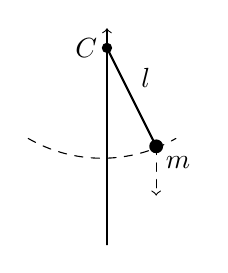
\begin{tikzpicture}[line cap=round,line join=round,scale=2.5]
        \node[left] at (0,1) {\(C\)}; 
        \fill (0,1) circle (0.75pt);

        \draw[-, thick] (0,1) -- (0.25,0.5);
        \fill (0.25,0.5) circle (1pt);
        \node[below right] at (0.25,0.5) {\(m\)}; 
        \node[above right] at (0.125,0.75) {\(l\)}; 

        \draw[->, thin, dashed] (0.25,0.5) -- (0.25,0.25);

        \draw[->] (0,0) -- (0,1.1);
        \draw[dashed] (-0.4,0.54) arc (-120:-60:0.75 and 0.75);
    \end{tikzpicture}
\end{center}

Chiaramente, \(\vec{F} = -mg \hat{z}\).
Il corpo è vincolato ad un percorso sul cerchio con centro il perno.
La posizione del punto è univocamente determinata dal raggio e dal suo angolo \(\theta\)
rispetto al perno.
Dal disegno notiamo che
\[
    F_N = T - mg \cos\theta
\]
mentre
\[
    F_T = -mg\sin\theta
\]
in quanto la tensione del filo non ha componenti tangenziali.
Sappiamo che per un moto arbitrario, la sua accelerazione può sempre essere
scritta in termini dell'accelerazione tangenziale e quella normale \(\vec{a} = \vec{a_T} + \vec{a_N}\).
Allora,
\[
    \begin{cases}
        m\frac{v^2}{R} = T-\cos\theta \\
        m\frac{dv}{dt} = -mg\sin\theta
    \end{cases}
\]
in questo caso il raggio di curvatura \(R\) è precisamente il raggio della circonferenza.
La distanza percorsa dal punto è \(s=l\Delta \theta\) e quindi
\[
    v = l \frac{d\theta}{dt}
\]
Sostituendo, troviamo la tensione del filo in funzione di \(\theta\),
dove \(\theta\) viene data dalla seconda equazione
\[
    \begin{cases}
        T = ml{\left(\frac{d\theta}{dt}\right)}^2 + \cos\theta \\
        \frac{d\theta^2}{dt^2} = -\frac{g}{l}\sin\theta
    \end{cases}
\]

Possiamo notare che il primo termine della tensione
si annulla ai due estremi. Il secondo termine
diventa negativo quando la pallina si trova sopra la semicirconferenza.
Infatti, in tale caso la tensione è negativa, e il cavo esercita tensione opposta
rispetto all'altro caso, in quanto deve contrastare il tentativo della pallina di accorciarlo.
Se la velocità iniziale è sufficientemente alta, la tensione è comunque positiva
se la pallina si trova nella parte superiore della circonferenza (come quando esegue un giro completo),
in tal caso la pallina sta comunque cercando di allungare il cavo.

Troviamo quindi la funzione \(\theta\). Per farlo, notiamo che
per piccoli angoli l'equazione è approssimativamente una funzione lineare.
Quindi,
\begin{align*}
    \theta = \theta_0 \cos(\omega t + \varphi), \quad \omega = \sqrt{\frac{g}{l}}
\end{align*}
con \(\varphi = 0\) (siccome la velocità iniziale è zero, il vincolo annulla la costante).
L'equazione senza l'approssimazione lineare non ha forma chiusa.

\pagebreak

\section{Esercizi}

\subsection{17 ottobre}

\sexercise{Un corpo viene lasciato cadere da una certa altezza
con velocità iniziale nulla: quanto tempo \(t\) si deve attendere perché
a parte da quell'istante il corpo percorra uno spazio di \(s= 20m\)
nel tempo \(\tau = 1s\)}{
    La funzione di caduta è data da \(s = \frac{1}{2}at^2 + v_0t + s_0\).
    Abbiamo allora 
    \begin{align*}
        20 &= \integral[t][t+1][v_0 + ax][x] \\
        20 &= \frac{1}{2}a{(t+1)}^2 - \frac{1}{2}at^2 \\
        40 &= a{(t+1)}^2 - at^2 \\
        40 &= a(t^2 + 2t + 1) - at^2 \\
        40 &= at^2 + 2at + a - at^2 \\
        40 &= 2at + a \\
        40 - a &= 2at \\
        t &= \frac{40 - a}{2a}
    \end{align*}
}

\sexercise{Il moto nel piano \(x\), \(y\) di una particella è definito da
\[
    \begin{cases}
        x = \alpha t^2  + \beta t \\
        y = \alpha t^2  - \beta t
    \end{cases}
\]
Con \(\alpha = 0.1 m/s^2\) e \(\beta = 1 m/s\).
Si calcolino i moduli della velocità e dell'accelerazione
all'istante \(\tau = 10s\)}{
    Calcoliamo le velocità
    \[
        \begin{cases}
            v_x = \frac{dx}{dt} = 2\alpha t + \beta \\
            v_y = \frac{dy}{dt} = 2\alpha t - \beta
        \end{cases}
    \]
    e le accelerazioni
    \[
        \begin{cases}
            a_x = \frac{dv_x}{dt} = 2\alpha \\
            a_y = \frac{dv_y}{dt} = 2\alpha
        \end{cases}
    \]
    Il modulo della velocità è pari a
    \begin{align*}
        |v| = \sqrt{v_x^2 + v_y^2}
        &= \sqrt{4\alpha^2 t^2 + 4\alpha\beta t + \beta^2 + 4\alpha^2 t^2 - 4\alpha\beta t + \beta^2} \\
        &= \sqrt{8\alpha^2 t^2 + 2\beta^2}
    \end{align*}
    Il modulo della accelerazione è pari a
    \begin{align*}
        |a| = \sqrt{8}\alpha
    \end{align*}
}

\sexercise{Un'automobile in moto con velocità di modulo \(v_0\)
comincia a frenare e, muovendosi di moto rettilineo, si arresta
in uno spazio \(l\).
Si determini l'accelerazione scalare media di frenamento nei tre casi seguenti:
}{
    \begin{enumerate}
        \item l'accelerazione scalare ha valore \(A\) costante nel tempo:
            Abbiamo che \(v = v_0 + At\) e \(s = v_0t + \frac{1}{2} A t^2\).
            Chiamiamo allora \(t^*\) il tempo per cui \(v=0\).
            Allora \(v_0 + At^* = 0 \implies t^* = - \frac{v_0}{A}\).
            %Allora \(l= v_0t^* + \frac{1}{2}At^*^2\)
            Sostituiamo \(t^*\) nell'accelerazione media
            \[
                a_m = \frac{v - v_0}{-t^*} = \frac{v_0}{-t^*} = A
            \]
        \item l'accelerazione dipende dalla velocità scalare con la legge:
        \(a = b(v + v_0)\). Dobbiamo trovare
        \begin{align*}
            \frac{dv}{dt} &= b(v + v_0)
        \end{align*} 
        quindi
        \begin{align*}
            v = ce^{\xi t} + V \qquad \frac{dv}{dt} = c\xi e^{\xi t} + V
        \end{align*}
        con \(V = -v_0\), \(\xi = b\) e \(c\) libera.
        Siccome \(v(0) = v_0\) allora \(c = 2v_0\) e quindi \(v(t) = v_0(2e^{b t} - 1)\).
        Per calcolare la posizione integriamo nuovamente
        \[
            \frac{ds}{dt} = v_0(2e^{bt} - 1)
        \]
        e allora
        \[
            s(t) = \frac{2v_0}{b}e^{bt} -v_0 t + s_0
        \]
        Siccome \(s(0) = 0 = -\frac{2v_0}{b}\), troviamo
        \[
            s(t) = \frac{2v_0}{b}(e^{bt} - 1) - v_0t
        \]
        Per il tempo di arresto abbiamo che \(v_0(2e^{bt} - 1) = 0\)
        e quindi \(t^* = - \frac{\ln 2}{b}\).
        Quindi \begin{align*}
            l &= s(t^*) = \frac{v_0}{b}\left(\ln 2 - 1\right) \\
            b &= \frac{v_0}{l} \left(\ln 2 - 1\right)
        \end{align*}
        Quindi l'accelerazione media è data da
        \[
            a_m = \frac{-v_0}{t^*} = \frac{v_0^2}{t} \frac{\ln 2 - 1}{\ln 2}
        \]
        \item l'accelerazione varia linearmente nel tempo \(a = \gamma t\):
            Integrando dobbiamo troviamo
            \begin{align*}
                v(t) &= v_0 + \frac{1}{2}\gamma t^2 \\
                s(t) &= v_0 t + \frac{1}{6}\gamma t^3
            \end{align*}
            siccome \(s_0 = 0\).
            \(\cdots\)
            Infine,
            \[
                a_m = \frac{2v_0^2}{3l}
            \]
    \end{enumerate}
}

\sexercise{Un corpo di piccole dimensioni
    viene lanciato verticalmente verso l'alto all'istante \(t=0\).
    Nella fase di salita e in quella successiva di discesa, l'oggetto passa dalla quota
    \(h\), rispetto alla posizione di lancio, agli istanti \(t_1\) e \(t_2\), rispettivamente:
    si dimostri che vale la relazione \(t_1t_2 = 2h/g\). Si trascuri l'effetto della
    resistanza dell'aria sul moto del corpo.}{
    La legge oraria è data da \(s(t) = v_0t + \frac{1}{2}at^2\).
    Dal testo abbiamo \(s(t_1) = s(t_2) = h\)
    e \(at^2 - 2v_0t + 2h = 0\).
    Le soluzioni sono
    \[
        t_1t_2 = \frac{v_0}{a} \pm \sqrt{\frac{v_0^2}{a^2} - \frac{2h}{g}}
    \]
    e quindi
    \[
        t_1t_2 = \frac{2h}{g}
    \]
}

\sexercise{Un corpo viene lanciato orizzontalmente
da altezza \(h_0\) rispetto al suolo, con velocità \(v_0\).
Trascurando la resistenza dell'aria, si calcoli:}{
    \begin{enumerate}
        \item la componente tangenziale \(a_T\) e quella normale \(a_N\)
        dell'accelerazione del corpo rispetto alla traiettoria, in un generico
        punto di altezza \(h\):
        abbiamo che \(P_0 = (0, h_0)\) e \(\vec{v_0} = (v_0, 0)\).
        Allora
        \[
            \begin{cases}
                a_x = 0 \\
                a_z = -g
            \end{cases}
        \]
        e
        \[
            \begin{cases}
                v_x = v_0 \\
                v_y = -gt
            \end{cases}
        \]
        e infine
        \[
            \begin{cases}
                x = v_0t \\
                z = h_0 - \frac{1}{2}gt^2
            \end{cases}
        \]
        Il vettore tangente è il vettore della velocità.
        Vogliamo trovare la legge che lega il tempo all'asse \(z\).
        Quindi \(\vec{v} = v_0\hat{x} - \sqrt{2g(h_0-z)}\hat{z}\)
        e \(|v| = \sqrt{v_0^2 + 2g(h_0 - z)}\).
        Se considiamo \(\alpha\) come l'angolo fra il vettore di gravitazione
        (asse x) e il vettore normale,
        \[
            \cos\alpha = \frac{\vec{v}\cdot\hat{x}}{|v|}
            = \frac{v_0}{\sqrt{v_0^2 + 2g(h_0 - z)}}
        \]
        che dipende da \(z\).
        Proiettiamo la gravità sulle sulle componenti, quindi
        \(a_T = g\sin\alpha\) e \(a_N = g\cos\alpha\), che si calcola facilmente
        con la relazione pitagorica del seno e coseno.
        \item lo spazio \(s\) percorso dal corpo dall'istante
        di lancio \(t=0\) a quello in cui tocca il suolo:
        \[
            \integral[0][\text{gittata}][\sqrt{1 + {\left(\frac{dz}{dx}\right)}^2}][x]
        \]
    \end{enumerate}
}

\sexercise{Una persona sale delle scale a chiocchiola
partendo dal piano terra all'istante \(t=0\).
La persona si mantiene a distanza costante \(r=2,\) dall'asse centrale delle scale e ogni
secondo sale uno scalino alto \(h=20cm\) e profondo \(d=20cm\).
Per studiare il moto della persona si adoperi:
\begin{enumerate}
    \item un sistema di coordinate cartesiane ortogonali;
    \item un sistema di coordinate cilindriche.
\end{enumerate}
Si ricavino nei due casi le equazioni della traiettoria, le legge orarie e le componenti della velocità
in funzione del tempo.}{
    \begin{enumerate}
        \item XXX;
        \item XXX.
    \end{enumerate}
}

\sexercise{Un punto percorre una traiettoria ellittica con modulo \(V\)
della velocità costante nel tempo. Rispetto a un sistema di assi cartesiani ortogonali l'equazione
dell'ellisse è
\[ \frac{x^2}{a^2} + \frac{y^2}{b^2} = 1 \]
con \(a\) e \(b\) indicando i semiassi. Si calcolino le componenti
\(x\) e \(y\) dell'accelerazione posseduta dal punto nella posizione \(P \equiv (x,y)\).}{
    XXX
}

\sexercise{Si consideri un moto piano tale per cui la velocità istantanea del piunto
materiale mantenga sempre lo stesso angolo \(\alpha \in (0, \frac{\pi}{2})\)
con la congiungente l'origine degli assi.
Si ricavi la traiettoria.}{
    XXX
}

\pagebreak

\subsection{24 ottobre}

\sexercise{
    Un osservatore lascia cadere un sasso in un pozzo al fine di
    rilevarne la profondità \(h\). Se l'intervallo di tempo intercorrente tra
    l'istante iniziale e quello in cui si ode il rumore prodotto dalla collissione
    del sasso con il fondo del pozzo è \(\Delta t\),
    quanto vale \(h\)? Si tenga conto della velocità del suono.
}{
    Abbiamo che il tempo di caduta più il tempo del suono
    è pari a
    \begin{align*}
        \sqrt{\frac{2h}{g}} + \frac{h}{v_\text{suono}}
        = \Delta t
    \end{align*}
    Risolvendo troviamo
    \begin{align*}
        \sqrt{\frac{2h}{g}}
        &= \Delta t - \frac{h}{v_s} \\
        \frac{2h}{g} &= {\left(\Delta t - \frac{h}{v_s}\right)}^2 \\
        \Delta t^2 + \frac{h^2}{v_s^2} - \frac{2\Delta t h}{s_v} &= \frac{2h}{g} \\
        0 &= h^2 - 2 \Delta t v_s h - \frac{2v_s^2h}{g} + \Delta t^2 v_s^2 \\
        0 &= h^2 - \left(2\Delta t v_s + \frac{2v_s^2}{g} + \Delta t^2 v_s^2\right) \\
        h_{1,2} &= \Delta t v_s + \frac{v_s^2}{g} \left(
            1 \pm \sqrt{1 + \frac{2\Delta t g}{v_s}}
        \right)
    \end{align*}
    Di cui consideriamo quella delle due che soddisfa l'equazione iniziale
    \[
        h = \Delta t v_s + \frac{v_s^2}{g} \left(
            1 + \sqrt{1 + \frac{2\Delta t g}{v_s}}
        \right)
    \]
}

\sexercise{Un proiettile viene sparato contro un bersaglio
    inizialmente posto ad'altezza \(h\) e che viene fatto cadere
    contemporaneamente allo sparo. Si dimostri che la condizione affinché il proiettile
    colpisca il bersaglio è che esso sia inizialmente puntato contro il bersaglio stesso.}{
    Se la distanza del proiettile è \(D\) allora dobbiamo dimostrare che
    \[
        \tan \alpha =\frac{h}{d}
    \]
    Le equazioni del moto del proiettile sono
    \begin{align*}
        \begin{cases}
            x_p = (v_0 \cos \alpha) t \\
            y_p = (v_0 \cos \alpha) t - \frac{1}{2}gt^2
        \end{cases}
    \end{align*}
    Le equazioni del moto del proiettile sono
    \begin{align*}
        \begin{cases}
            x_b = D \\
            y_b = h - \frac{1}{2}gt^2
        \end{cases}
    \end{align*}
    Dobbiamo imporre il fatto che i due oggetti si incontrino in un certo momento.
    Quindi \(x_p = x_b\) e \(y_p = y_b\).
    Troviamo allora
    \begin{align*}
        \begin{cases}
            (v_0 \cos \alpha) t = D \\
            (v_0 \sin \alpha) t = h
        \end{cases}
    \end{align*}
    Senza risolvere le equazioni, notiamo che
    la divisione porta alla nostra condizione
    \[
        \frac{v_0 t \sin \alpha}{v_0 t \cos \alpha} = \frac{h}{D}
    \]
}

\sexercise{Un punto materiale si muove lungo un arco di circonferenza di raggio \(R\)
con la seguente legge oraria:
\[s = s_0\cos \omega t\]
dove \(s\) è l'ascissa curvilinea ed \(s_0\) e \(\omega\)
sono costanti assegnate. Trovare la velocità angolare
e le componenti normale e tangenziale dell'accelerazione.}{
    Abbiamo che \(s = R \theta\). Allora
    \begin{align*}
        R\theta &= R \theta_0 \cos(\omega t) \\\
        \theta &= 0_0 \cos(\omega t)
    \end{align*}
    e quindi la velocità angolare è data da
    \begin{align*}
        \Omega = \frac{d\theta}{dt} = -w \theta_0 \sin(\omega t)
    \end{align*}
    L'accelerazione è data dalla componente normale
    \[
        a_N = \frac{v^2}{R}
    \]
    e
    \[
        a_T = \frac{dv}{dt}
    \]
    Siccome \(v=\Omega R\), abbiamo
    \[
        v = -\omega R \theta_0 \sin(\omega t)
    \]
    e
    \begin{align*}
        \begin{cases}
            a_N = \frac{\omega^2 R^2 \theta_0^2 \sin^2(\omega t)}{R} \\
            a_T = -\omega^2 R \theta_0 \cos(\omega t) = -\omega^2 s
        \end{cases}
    \end{align*}
}

\sexercise{Due aeroplani \(A\) e \(B\) hanno velocità opposte
di modulo \(v\) e le loro traiettorie sono due rette parallele distanti \(d\)
Sia \(t=0\) l'istante in cui la retta \(AB\) sarebbe perpendicolare alle due traiettorie.
L'asse del cannone montato su \(A\) forma un angolo \(\alpha\)
con l'asse dell'aereo e i proiettili vengono sparati con velocità di modulo \(v_r\)
relativa ad \(A\). A quale istante \(t^*\) l'aereo \(A\) deve sparare affinché
l'aereo \(B\) venga colpito? Non si consideri l'Accelerazione di gravità.}{
    La legge oraria per \(A\) per \(t < t^*\) è data da
    \begin{align*}
        \begin{cases}
            x_A(t) = vt \\
            y_A(t) = 0
        \end{cases}
    \end{align*}
    mentre per \(t \geq t*\) consideriamo il moto del proiettile
    \begin{align*}
        \begin{cases}
            x_P(t) = vt^* + (v_r \cos \alpha + v)(t - t^*) \\
            y_P(t) = (v_r \sin \alpha)(t - t^*)
        \end{cases}
    \end{align*}
    La legge oraria di \(B\)
    \begin{align*}
        \begin{cases}
            x_B(t) = -vt \\
            y_B(t) = d
        \end{cases}
    \end{align*}
    Allora dobbiamo eguagliare le leggi orarie
    \begin{align*}
        \begin{cases}
            x_P(t) = x_B(t) \\
            y_P(t) = y_B(t) \\
        \end{cases}
    \end{align*}
    quindi troviamo
    \begin{align*}
        \begin{cases}
            vt^* + (v+v_r \cos \alpha)(t-t^*) = -vt \\
            (v_r \sin \alpha)(t-t*) = d
        \end{cases}
    \end{align*}
    Dalla seconda ricaviamo \(t-t^* = \frac{d}{v_r \sin \alpha}\).
    Sostituiamo questo valore nella prima
    \begin{align*}
        vt^* + (v + v_r \cos\alpha) \frac{d}{v_r \sin\alpha} &= -vt \\
         &= -v(t-t^*) - vt^* \\
         &= -v(t-t^*) - vt^* \\
         -\frac{d(2v + v_r\cos\alpha)}{2vv_r\sin\alpha} &= t^*
    \end{align*}
}

\sexercise{Un'automobile parte da ferma con moto uniformemente accelerato con
accelerazione \(a\). Dopo un tempo \(\tau\) si lancia un proietile che si può
supporre in moto con velocità costante \(v_0\). Determinare la minima velocità
\(v_0\) necessaria a colpire l'automobile, in funzione di \(a\) e \(\tau\).
Si pu?o considerare il moto puramente unidimensionale.}{
    Le legge orarie sono
    \begin{align*}
        \begin{cases}
            x_A(t) = \frac{1}{2}at^2 \\
            x_P(t) = v_0(t-\tau)
        \end{cases}
    \end{align*}
    Abbiamo allora \(x_A(t) = x_P(t)\)
    \begin{align*}
        \frac{1}{2}at^2 &= v_0(t-\tau) \\
        \frac{1}{2}at^2 + v_0\tau &= v_0t
    \end{align*}
    e quindi
    \begin{align*}
        t_{1,2} = \frac{v_0}{a} \pm \sqrt{\frac{v_0^2}{a^2} - \frac{2v_0\tau}{a}}
    \end{align*}
    e la condizione è data dal discriminante
    \[
        \frac{v_0^2}{a^2} > \frac{2v_0\tau}{a}
        \implies
        v_0 > 2a\tau
    \]
}

\sexercise{Un treno in moto rettilineo uniforme con una velocità di modulo \(v\)
rallenta bruscamente con decelerazione costante di modulo \(A\):
come conseguenza, una valigia, posata in bilico sul portapacchi, cade e finisce sul pavimento del treno.
Si determini la traiettoria della valigia come apapre a un osservatore \(O\)
fermo a terra e a uno \(O'\) sul treno.}{
    La legge oraria inerziale della valigia è data da
    \begin{align*}
        \begin{cases}
            x = v_0 t \\
            y = h - \frac{1}{2}gt^2
        \end{cases}
    \end{align*}
    Per il riferimento non inerziale abbiamo \(\vec{a} = \vec{a'} + \vec{\Delta}_\text{trascinamento}\),
    quindi \(\vec{a'} = \vec{g} - \vec{A}\).
    \begin{align*}
        \begin{cases}
            \frac{d^2x'}{dt^2} = A \\
            \frac{d^2y'}{dt^2} = -g
        \end{cases}
    \end{align*}
    Da queste due leggi ricaviamo le leggi orarie
    \begin{align*}
        \begin{cases}
            x' = \frac{1}{2}At^2 \\
            y' = -\frac{1}{2}gt^2 + h
        \end{cases}
    \end{align*}
    e da cui troviamo la traiettoria \(y' = h - \frac{g}{A}x'\)
    che è una retta.
}

\pagebreak

\subsection{31 ottobre}

\sexercise{Un uomo di trova su un ascensore che sale a velocità
costante \(V_0\). Egli lancia ua pallina verticalmente verso l'alto con velocità \(v_0\)
relativa all'ascensore:
\begin{enumerate}
    \item determinare dopo quanto tmepo la pallina ritorna nella mano dell'uomo;
    \item rispondere alla domanda precedente nel caso in cui l'ascensore abbia una
    accelerazione diretta verso l'alto pari a \(A_\text{asc}\).
\end{enumerate}
Suggerimento: provare a risolvere il problema in due modi:
\begin{enumerate}
    \item usando le leggi dei moti relativi;
    \item usando le leggi del moto dei due corpi viste dal sistema di riferimento
    della terra ferma. Verificare che i risultati siano gli stessi.
\end{enumerate}}{
    XXX
}

\sexercise{Una piattaforma ruota con velocità angolare
\(\omega\) intorno a un asse centrale verticale.
All'istante \(t = 0\), una pallina viene lanciata orizzontalmente con velocità \(v_0\)
dal centro della piattaforma; l'attrito che la pallian incontra è trascurabile,
cosiché essa si muova rispetto alla terra di moto rettilineo uniforme con velocità \(v_0\).
Si determini l'accelerazione della pallina, a un generico istante, rispetto a un sistema di riferimento
solidale alla piattaforma.}{
    XXX
}

\sexercise{Sia \(\vec{g_0}\) l'accelerazione di gravità che si misurerebbe in corrispondenza
di un punto \(P\) della superficie terrestre qualore la Terra non fosse in rotazione;
si determini l'accelerazione di gravità efficace misurata da un osservatore solidale con la Terra.
Si calcoli inoltre la deviazione subita da un corpo in caduta libera dovuta all'accelerazione di Coriolis, all'equatore.}{
    XXX
}

\sexercise{Su di un corpo di massa \(m\) agisce una forza funzione del tempo data da:
\(F = F_0 - \alpha t\), con \(F_0\) ed \(\alpha\) costanti assegnate.
All'istante iniziale il corpo transita per l'origine con velocità \(v_0\).
Si trovino velocità e posizione in funzione del tempo.}{
    XXX
}

\sexercise{Una particella si muove sotto l'azione di una forza \(\vec{F} = \vec{u} \times \vec{c}\),
dove \(\vec{c}\) è un vettore costante. SI trovino traiettoria e legge oraria.}{
    XXX
}

\sexercise{Due rimorchiatori trainano un battello tramite cavi d'acciaio, fissati a prua del battello.
L'angolo tra i cavi e l'orizzontale è \(60^\circ\),
e la tensione è pari a \(2\times 10^5 N\) per ciascuno dei cavi.
Si trovi la forza resistente dovuta all'acqua, se il battello si muove di moto uniforme.}{
    XXX
}

\end{document}